\section{Pianificazione}
Lo sviluppo del progetto viene organizzato e suddiviso nelle seguenti fasi:
\begin{itemize}
\item \textbf{Analisi preliminare};
\item \textbf{Progettazione e codifica Proof of Concept};
\end{itemize}

%fase di Analisi preliminare

\subsection{Analisi preliminare}
Questo periodo comincia nel momento in cui vengono assegnati i capitolati e termina con l'inizio del periodo di Progettazione e codifica Proof of Concept.\\
\begin{center}
\textbf{periodo:} dal 5-11-2022 al 14-12-2022\\
\end{center}
In questo periodo ci si concentra nel definire il way of working, creare tutta la documentazione necessaria e fare un analisi approfondita del capitolato scelto.  Questo periodo viene suddiviso nelle attività trattate nella seguente sezione.

\subsubsection{Attività}
\begin{itemize}
\item \textbf{Norme di progetto:} vengono individuati gli strumenti e le linee guida da seguire durante lo sviluppo del progetto;
\item \textbf{Piano di progetto:} documento in cui viene definita la pianificazione del progetto e le sue varie fasi,  in più fornisce un preventivo per ogni fase pianificata ed il totale costo ed ore necessario per la realizzazione del progetto;
\item \textbf{Analisi dei requisti:} viene eseguito uno studio approfondito dei requisti del capitolato scelto,  di conseguenza si costruisce un diagramma dei casi d'uso e un diagramma delle attività;
\item \textbf{Glossario: } documento contenente la descrizione di termini di dominio del progetto, il glossario sarà continuamente aggiornato in base alla necessità.
\end{itemize}

\subsubsection{Periodi}
La fase di Analisi preliminare sarà suddivisa nei seguenti periodi:
\begin{itemize}
\item \textbf{Periodo 1:} \textit{dal 5-11-2022 al 16-11-2022},  pianificazione del periodo di Analisi preliminare,  suddivisone dei ruoli fra i componenti del gruppo,  prima stesura delle norme di progetto, viene effettuata un'analisi dei rischi.  Inoltre ci sarà la continua stesura di verbali dopo ogni incontro con il gruppo e con il proponente;
\item \textbf{Periodo 2:} \textit{dal 16-11-2022 al 7-12-2022},  analisi dei requisti del capitolato scelto,  prima stesura del glossario, stesura del piano di progetto con rispettivo preventivo della fase di Analisi preliminare.  I componenti del gruppo si impegnano a studiare le tecnologie necessarie per il compimento del progetto. Si continua a lavorare nei documenti redatti nei periodi precedenti e continuano ad essere prodotti verbali riguardanti le riunioni;
\item \textbf{Periodo 3: } \textit{dal 7-12-2022 al 14-12-2022}, stesura del documento \textit{Analisi dei Requisti}. Vengono completati eventuali documenti in ritardo e avviene la verifica dei documenti che la necessitano.
\end{itemize}

\begin{figure}[H]
    \centering
    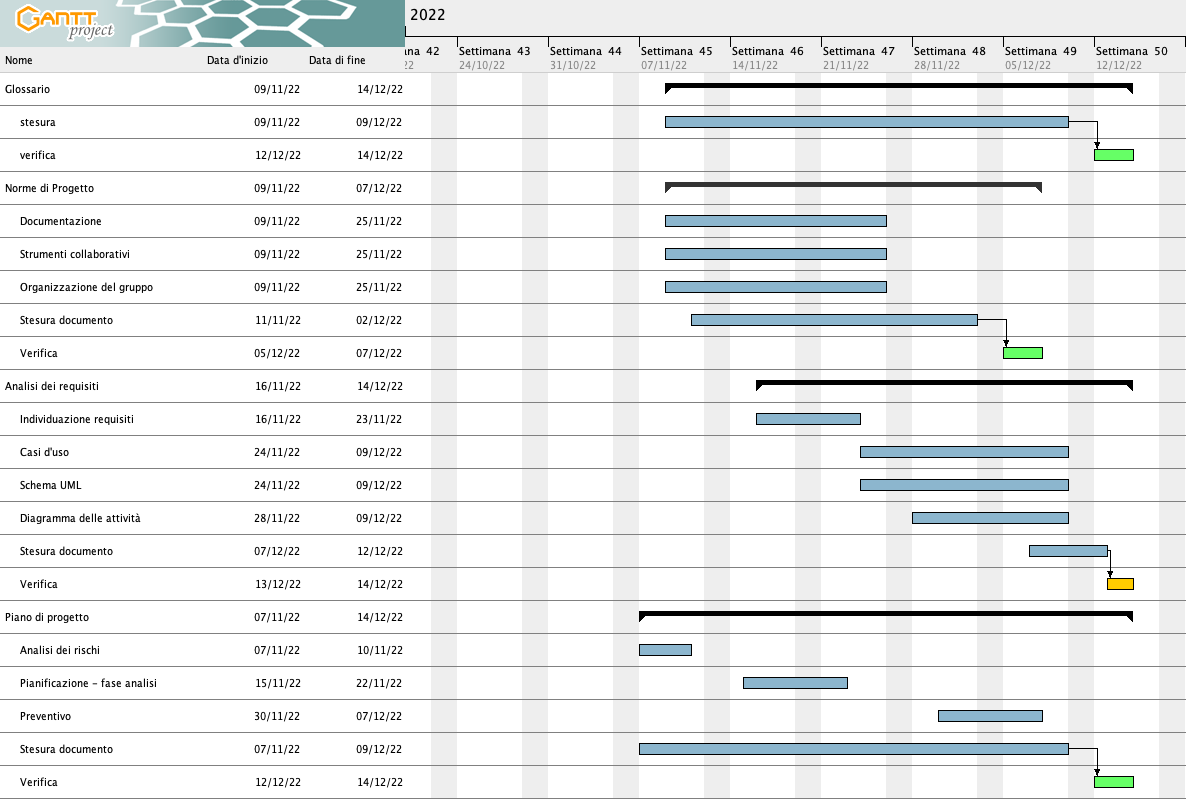
\includegraphics[scale=0.38]{image/analisi_preliminare_gantt.png}
    \caption{Diagramma di Gantt fase di Analisi preliminare}
\end{figure}
\pagebreak
%fase PoC

\subsection{Progettazione e codifica Proof of Concept}
Questo periodo comincia al termine del periodo di Analisi preliminare e termina con l'inizio della codifica del Proof of Concept.\\
\begin{center}
\textbf{periodo:} dal 15-12-2022 al 16-01-2023\\
\end{center}
Questo periodo viene dedicato al completamento delle attività arretrate, per poi concentrarsi sulla 
progettazione e la codifica del Proof of Concept. Si va inoltre avanti con la stesura 
della documentazione. Questo periodo viene suddiviso nelle attività trattate nella seguente sezione.

\subsubsection{Attività}
\begin{itemize}
\item \textbf{Glossario:} il documento viene costantemente aggiornato con nuovi termini;
\item \textbf{Piano di progetto:} viene aggiunta la pianificazione del periodo, il preventivo e il consultivo;  
\item \textbf{Analisi dei requisti:} si continua la stesura del documento, completando le attività arretrate dal periodo precedente;
\item \textbf{Piano di Qualifica:} documento nel quale vengono stabiliti gli standard di qualità di processo e di prodotto;
\item \textbf{Norme di Progetto:} vengono aggiunte nuove norme relative alla documentazione e alle metriche utilizzate nel \textit{Piano di Qualifica};
\item \textbf{Proof of Concept:} a seguito di uno studio individuale delle tecnologie, si inizia a progettare e realizzare il Proof of Concept, una versione semplice, ma dimostrativa, del prodotto finale, per 
capire se è fattibile e darne una prova al proponente.
\end{itemize}

\subsubsection{Periodi}
La fase di Progettazione e codifica Proof of Concept sarà suddivisa nei seguenti periodi:
\begin{itemize}
\item \textbf{Periodo 1:} \textit{dal 15-12-2022 al 21-12-2022}, pianificazione del periodo corrente con relativo preventivo, completamento attività arretrate 
(stesura del documento \textit{Analisi dei Requisiti}). continua lo studio individuale delle tecnologie da utilizzare;
\item \textbf{Periodo 2:} \textit{dal 22-12-2022 al 04-01-2023},  stesura del documento \textit{Piano di Qualifica}. Inizia la progettazione del Proof of Concept, si continua la stesura e la verifica dei documenti;
\item \textbf{Periodo 3:} \textit{dal 05-01-2023 al 16-01-2023}, continua la progettazione e inizia la codifica del Proof of Concept. Si procede nella stesura e nella verifica della documentazione.
\end{itemize}

\begin{figure}[H]
    \centering
    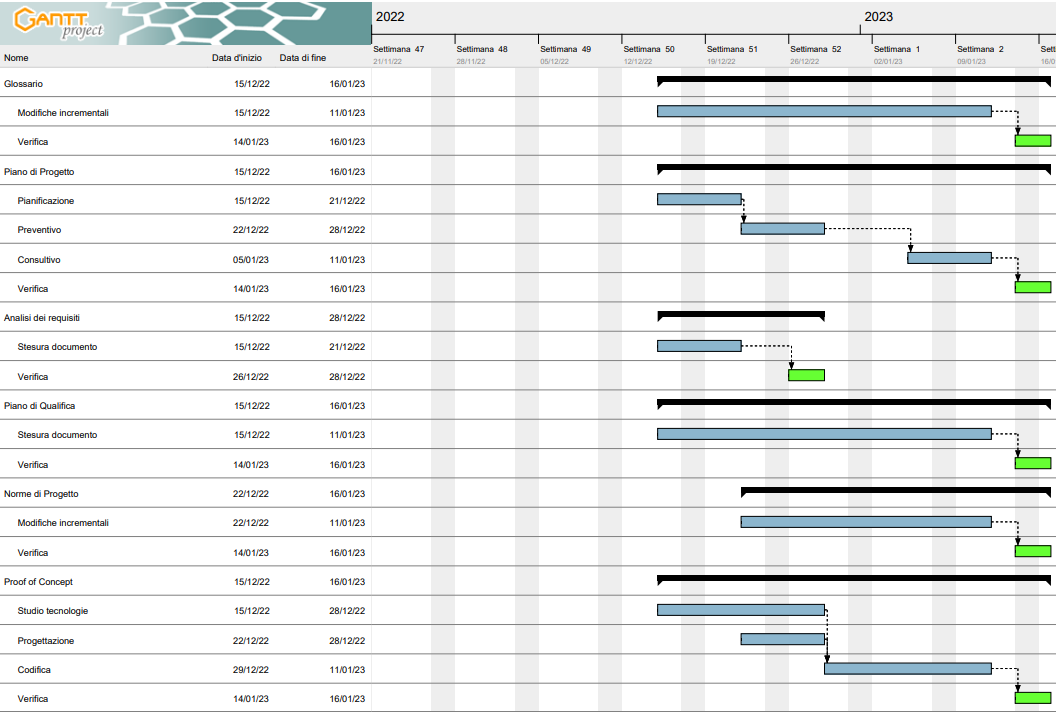
\includegraphics[scale=0.75]{image/gantt_poc.png}
    \caption{Diagramma di Gantt fase di Progettazione e codifica Proof of Concept}
\end{figure}
\pagebreak